% --- [ Control Flow Analysis Terminology ] ------------------------------------

\subsection{Control Flow Analysis Terminology}
\label{app:control_flow_analysis_terminology}

% ~~~ [ Basic Block ] ~~~~~~~~~~~~~~~~~~~~~~~~~~~~~~~~~~~~~~~~~~~~~~~~~~~~~~~~~~

\subsubsection{Basic Block}

A basic block is a sequence of non-branching instructions terminated by a branching instruction, where incoming branches may only target the first instruction of the basic block and outgoing branches may only leave from the last instruction of the basic block; as illustrated in listing \ref{lst:basic_block}.

\lstinputlisting[language=nasm, style=nasm, label={lst:basic_block}, caption={Examples of basic blocks in x86 assembly.}]{inc/appendices/vocabulary/basic_block.asm}

% ~~~ [ Control Flow Graph ] ~~~~~~~~~~~~~~~~~~~~~~~~~~~~~~~~~~~~~~~~~~~~~~~~~~~

\subsubsection{Control Flow Graph}

A control flow graph $G = (V, E, r)$ is a directed graph rooted at $r$ with vertex set $V$ and edge set $E$, where $r$ denotes the entry point of execution, $v \in V$ denotes a basic block and $(u, v) \in E$ denotes the transfer of control of execution from $u$ to $v$. The corresponding control flow graph of the x86 assembly example in listing \ref{lst:basic_block} is presented in figure \ref{fig:control_flow_graph}.

\begin{figure}[htbp]
	\centering
	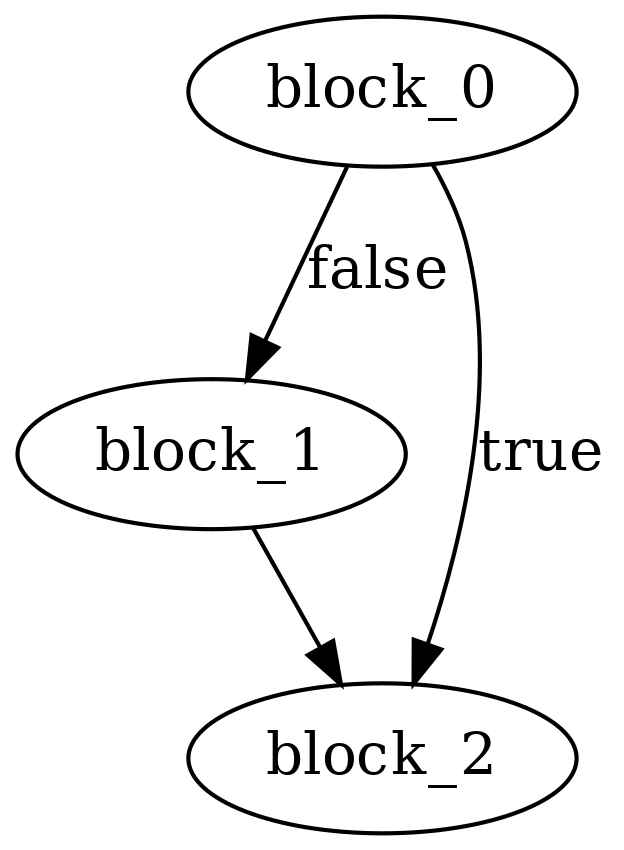
\includegraphics[width=0.2\textwidth]{inc/appendices/vocabulary/control_flow_graph.png}
	\caption{Control flow graph rooted at \texttt{block\_0} corresponding to the x86 assembly example in listing \ref{lst:basic_block}.}
	\label{fig:control_flow_graph}
\end{figure}
